% By zmienic jezyk na angielski/polski, dodaj opcje do klasy english lub polish
\documentclass[polish,12pt]{aghthesis}
\usepackage[utf8]{inputenc}
\usepackage{url}
\usepackage{listings}

\author{Przemysław Dąbek, Roman Janusz\\ Tomasz Kowal, Małgorzata Wielgus}

\title{Platforma do automatycznych aktualizacji oprogramowania na urządzeniach zdalnych. - dokumentacja techniczna}

\supervisor{dr inż. Wojciech Turek}

\date{2012}

% Szablon przystosowany jest do druku dwustronnego,
\begin{document}

\maketitle





\section{Cel prac i wizja produktu}
%\section{Project goals and vision}
\label{sec:cel-wizja}
\subsection{Wstęp}
Celem niniejszego rozdziału jest ogólne nakreślenie i scharakteryzowanie wymagań stawianych systemowi ze względu na jego przeznaczenie i sposób użycia, a także określenie najważniejszych założeń jego realizacji.
Wszelkie decyzje implementacyjne nie są tu podejmowane i opisane zostaną w następnych rozdziałach.
\subsection{Słownik}
\begin{tabular}{| l | p{9cm} |}
  \hline
  Pojęcie & Definicja \\ \hline
  Serwer główny & Serwer, do którego łączą się urządzenia zdalne w celu przekazania zebranych danych.\\ \hline
  Urządzenie zdalne & Urządzenie znajdujące się w terenie, może mieć ograniczone zasoby sprzętowe oraz zawodne połączenie z serwerem głównym.\\ \hline
  Repozytorium oprogramowania & Specjalny serwer platformy, na którym znajduje się software.\\ \hline
  Węzeł & Środowisko uruchomieniowe Erlanga z nadaną nazwą.\\ \hline
  Sieć węzłów & Węzły połączone w sieć za pomocą Erlangowych mechanizmów.\\ \hline
  Aplikacja & Program implementujący wzorzec projektowy OTP Application. \\ \hline
\end{tabular}

\subsection{Odnośniki}
\begin{itemize}
\item \url{http://beagleboard.org/} - opis przykładowego urządzenia, z którym powinna współpracować platforma
\item \url{http://alancastro.org/2010/05/01/erlang-application-management-with-rebar.html} - Rebar: narzędzie do budowania aplikacji
\item \url{http://www.angstrom-distribution.org/} - Dystrybucja Linuxa na urządzenia wbudowane
\item \url{http://erlang.org/pipermail/erlang-questions/2011-April/057375.html} oraz
\item \url{https://fedoraproject.org/wiki/Summer_coding_ideas_for_2011#Better_Erlang_support} - Projekt dotyczący stworzenia paczek rpm z aplikacji Erlangowych
\end{itemize}

\subsection{Opis problemu}
Problem: Duża ilość zdalnych urządzeń rozmieszczonych w terenie. Urządzenia komunikują się przez zawodną sieć. Na różnych urządzeniach działają różne wersje aplikacji. Zachodzi potrzeba aktualizacji oprogramowania na grupie urządzeń. Rozwiązanie: Platforma umożliwi monitorowanie oraz aktualizację wersji aplikacji na grupach urządzeń.

\subsection{Opis użytkownika i zewnętrznych podsystemów}
Użytkownikiem systemu jest osoba odpowiedzialna za oprogramowanie w systemie składającym się z urządzeń zdalnych. System składa się z dużej liczby tych urządzeń, które mogą mieć mocno ograniczone zasoby sprzętowe (np. Beagleboard). Urządzenia mogą mieć różne architektury. Urządzenia będą łączyć się z serwerem głównym, do którego przesyłają zebrane dane. Komunikacja odbywa się za pomocą zawodnego połączenia (np. GSM).

\subsection{Opis produktu}
Produkt będzie składał się z serwera zawierającego repozytorium oprogramowania. Serwer będzie miał za zadanie monitorować jakie wersje aplikacji znajdują się na konkretnych urządzeniach i grupach urządzeń. Zostanie udostępniony interfejs webowy, dzięki któremu można będzie wybrać urządzenia (lub ich grupy), na których chcemy przeprowadzić aktualizację i sprawdzić jakie aplikacje są zainstalowane. Ponieważ nie zawsze możliwe jest połączenie z wybranym urządzeniem, serwer powinien przechowywać jego stan. W momencie uzyskania połączenia z urządzeniem serwer powinien wykonać zaplanowane aktualizacje.

\subsection{Wymagania funkcjonalne i ich priorytety}
Platforma:
\begin{itemize}
\item monitoruje, czy dane urządzenie jest dostępne \emph{10}
\item monitoruje zainstalowane aplikacje oraz ich wersje na urządzeniach \emph{10}
\item rejestruje urządzenia \emph{10}
\item pozwala na definiowanie grup urządzeń \emph{4}
\item umożliwia aktualizację i instalację aplikacji na pojedynczych urządzeniach \emph{8}
\item umożliwia aktualizację i instalację aplikacji na grupach urządzeń \emph{5}
\item umożliwia aktualizację i instalację za pomocą systemowych narzędzi takich jak apt, yum, port \emph{7}
\item umożliwia Hot Code Update dla aplikacji Erlangowych \emph{2}
\item umożliwia aktualizację aplikacji Erlangowej działającej na sieci połączonych węzłów \emph{1}
\item webowy interfejs użytkownika \emph{3}
\item umożliwia tworzenie paczek aplikacji dedykowanych dla platformy wraz ze skryptami instalacyjnymi \emph{6}
\end{itemize}

\subsection{Inne wymagania dotyczące produktu}
\begin{itemize}
\item Obsługa między 1000 - 10000 urządzeń
\item Obsługa różnych architektur i systemów operacyjnych
\item Prawidłowe działanie w przypadku zrywających się połączeń
\item Wymagania stawiane dokumentacji:
  \begin{itemize}
  \item Podręcznik użytkownika
  \item Podręcznik instalacji i konfiguracji.
  \item Dokumentacja techniczna - dokumentacja kodu, opis testów.
  \end{itemize}
\end{itemize}

\subsection{Wstępna analiza ryzyka}
\begin{itemize}
\item brak czasu ze względu na inne projekty na studiach, prawdopodobieństwo \emph{10}, skutki \emph{8}
\item brak możliwości przetestowania na dużej ilości urządzeń zdalnych, prawdopodobieństwo \emph{10}, skutki \emph{3}
\item nieznajomość niektórych narzędzi systemowych do aktualizacji oprogramowania, prawdopodobieństwo \emph{5}, skutki \emph{6}
\item brak doświadczenia w pisaniu oprogramowania na niektóre architektury, prawdopodobieństwo \emph{8}, skutki \emph{5}
\item brak doświadczenia z używaniem sieci innych niż Ethernet, prawdopodobieństwo \emph{6}, skutki \emph{6}
\end{itemize}

\section{Koncepcja Architektury}
\subsection{Przegląd technologii do zastosowania w platformie}
\subsubsection{Technologia do stworzenia graficznego interfejsu użytkownika}
Pod uwagę brano:
\begin{itemize}
\item Ruby on Rails z połączeniem Erlectricity
\item Yaws
\item Mochiweb
\item Webmachine
\item Nitrogen
\item Zotonic – CMS i framework
\end{itemize}

RoR: Według przykładów najpierw uruchamiany był proces erlanga, który dopiero wywoływał program w Rubym i dopiero wtedy zachodziła komunikacja. Nie można jednym procesem erlangowym dopiąć się do jednej klasy aplikacji w Ruby on Rails.

Yaws: Serwer napisany całkowicie w Erlangu. Tworzenie interfejsu odbywa się w specjalnym dialekcie eHTML. Wydaje się być najlepszym rozwiązaniem.

Mochiweb: jest narzędziem do budowania własnych lekkich serwerów http. Zbudowanie własnego serwera od zera dodałoby niepotrzebny dodatkowy stopień do złożoności problemu.

Webmachine: Zestaw narzędzi do tworzenia web serwisów opartych o technologię REST. Prawdopodobnie nie będzie nam potrzebny.

Nitrogen: Jest to framework do tworzenia aplikacji webowych w erlangu. Do tego potrzebny byłby jeszcze serwer.

Zotonic: Framework i CMS w erlangu. Aby dopisać obsługę serwera trzeba napisać dodatkowe moduły i poznać jego strukturę.

\subsubsection{Komunikacja między urządzeniem zdalnym, a głównym serwerem platformy:}
\begin{itemize}
\item wywoływanie poleceń przez SSH
\item komunikacja przez socket TCP
\item komunikacja między węzłami sieci erlanga
\item web service
\end{itemize}

SSH: Połączenie może być w każdej chwili zrywane, co może skutkować nieprzewidywalnym zachowaniem. Wymaga również zmian konfiguracji w systemie operacyjnym zdalnego urządzenia (użytkownik, klucz, plik sudoers).

TCP: Rozwiązanie o najmniejszym narzucie komunikacyjnym. Łatwe do obsłużenia w erlangu za pomocą gen\_tcp. Wymagana samodzielna obsługa zrywanych połączeń, zaprojektowanie własnego formatu wiadomości. Wydaje się być najlepszym rozwiązaniem.

Węzły sieci erlanga: Po połączeniu z danym urządzeniem połączenie jest stale utrzymywane, co nie jest pożądane (ani nawet możliwe) w naszym przypadku.

Web Serwisy: Powodują duży narzut komunikacyjny, a ponieważ zakładamy dużą liczbę urządzeń, chcieliśmy tego uniknąć.

\subsubsection{Język programowania do implementacji klienta oraz serwera}
W związku z tym, że wybraliśmy komponenty, które są napisane w erlangu, to aby uniknąć problemów na styku różnych technologii, postanowiliśmy napisać zarówno klienta, jak i serwer w erlangu.

\subsubsection {Wybór bazy danych}
\begin{itemize}
\item mnesia
\item MySQL
\item ewentualnie inne relacyjne bazy danych
\end{itemize}

\centerline{
	% skalujemy 90%
	\scalebox{0.5}{
		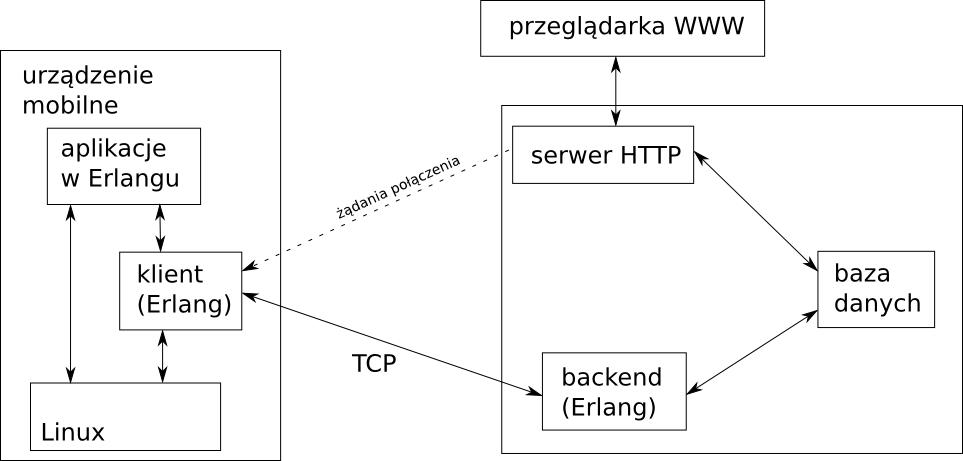
\includegraphics{scheme.png}
	}
}

\subsection{Opis diagramu}
Na diagramie prostokątem po lewej zaznaczono urządzenie mobilne. Działa na nim pewna dystrybucja linuxa. Uruchomiona jest maszyna wirtualna erlanga wraz z działającą aplikacją (aplikacjami). Dodatkowo powinien zostać uruchomiony klient naszej platformy.

Po prawej stronie znajdują się (od góry) administrator korzystający z webowego interfejsu, serwer HTTP (mochiweb), backend platformy zaimplementowany w erlangu, baza danych i repozyterium pakietów.

\subsection{Obsługa przykładowego żądania użytkownika}
\begin{itemize}
\item żądanie z przeglądarki przesyłane jest do serwera http
\item jest interpretowane i wywoływane są odpowiednie funkcje backendu platformy
\item backend czeka na połączenie ze zdalnym urządzeniem, urządzenie łączy się z serwerem głównym co określony interwał czasu
\item przez klienta na zdalnej maszynie odbierane jest polecenie (na przykład ściągnięcia nowej wersji oprogramowania)
\item uruchamiane są odpowiednie polecenia systemu linux (np. apt-get)
\item po ich zakończeniu klient wysyła powiadomienie o wykonaniu operacji do serwera
\item serwer po odebraniu wiadomości zapisuje nowy stan urządzenia w bazie
\end{itemize}




\section{Rozszerzona koncepcja architektury - opis komponentów platformy}

\subsection{Backend (sup\_server\_management)}
Aplikacja erlangowa, która odpowiada za całość automatycznego zarządzania urządzeniem. Podejmuje wszystkie decyzje o tym, jakie czynności ma wykonać urządzenie oraz zleca ich wykonanie. Obejmuje to przede wszystkim:

\begin{itemize}
\item aktualizację oprogramowania
\item monitorowanie stanu urządzenia
\item zarządzanie konfiguracją urządzenia
\end{itemize}

Decyzje o czynnościach, które należy wykonać na urządzeniu podejmowane są na podstawie danych wyciągniętych z bazy danych na serwerze oraz wiadomości przesłanych bezpośrednio przez urządzenie podczas połączenia.

Dane w bazie mogą pochodzić od serwera zarządzającego lub są dodane przez użytkownika za pomocą interfejsu webowego.

Na każde połączenie urządzenia z serwerem spawnowany jest jeden proces erlangowy.

\subsection{Klient serwera zarządzającego (na urządzeniu zdalnym)}
Jest to aplikacja erlangowa, która komunikuje się z serwerem zarządzającym i wykonuje zlecone przez niego zadania na urządzeniu zdalnym. Klient nie podejmuje samodzielnie żadnych decyzji związanych czynnościami, które należy wykonać, wykonuje jedynie polecenia przychodzące z serwera i odpowiada odsyłając dokładne rezultaty wykonywanych poleceń. W związku z tym, że nie możemy zakładać dostępności urządzenia zdalnego z serwera, przyjęliśmy, że połączenie zawsze inicjowane jest przez klienta. Nie znaczy to, że nie zakładamy żadnej możliwości notyfikacji klienta, jednak nie możemy przyjąć żadnej uniwersalnej metody takiej notyfikacji. Jeżeli mamy możliwość połączenia się z urządzeniem przez SSH, możemy zlecić mu natychmiastowe połączenie do serwera. Preferowanym sposobem wykonania żądania połączenia jest wysłanie go bezpośrednio z serwera http na żądanie interfejsu użytkownika.

\subsection{Interfejs pomiędzy serwerem, a klientem}
Klient komunikuje się przede wszystkim z bazą danych na serwerze i zapisuje w niej dane, na podstawie których serwer podejmuje decyzje, co do wykonywanych czynności.

\subsection{Serwer ftp}
Służy do przechowywania archiwów z erlangowymi releasami.

\subsection{Baza danych (Mnesia)}
Stanowi element łączący serwer zarządzający i serwer http.

\subsection{Graficzny interferjs użytkownika (serwer http - Mochiweb)}
Służy do wyświetlania stanu urządzeń zapisanego w bazie danych oraz zapisywania do bazy poleceń dla konkretnych urządzeń. Serwer nie komunikuje się bezpośrednio z serwerem zarządzającym. Robi to pośrednio przez zapisywanie żądań do bazy danych. W związku z tym wykonanie żądań nie jest natychmiastowe. Jeżeli zależy nam, aby zmiany odniosły skutek natychmiastowy, należy wykorzystać mechanizm żądania połączenia (connection request). Proces wygląda następująco:
\begin{itemize}
\item Użytkownik podłącza się do node'a Erlangowego i wywołuje funkcję sup\_server\_management:trigger\_session(Reason).
\item Urządzenie rozpoczyna komunikację z serwerem zarządzającym
\item Serwer zarządzający zleca mu zadania na podstawie danych w bazie
\end{itemize}
Wraz z żądaniem połączenia można przesłać token. Klient przesyła ten token do serwera zarządzającego. Jest to dodatkowa informacja, na podstawie której serwer zarządzający wybiera zadania. W ten sposób można połączyć konkretne zadania z danym żądaniem połączenia.

\section{Szczegóły protokołu komunikacyjnego i sesji zarządzania}
Połączenie nawiązywane jest za pomocą tcp (gen\_tcp). Przesyłane wiadomości są termami erlangowymi serializowanymi za pomocą funkcji term\_to\_binary/1. Komunikację obejmującą jedno połączenie nazywamy sesją zarządzania.

\subsection{Szczegóły przebiegu sesji z punktu widzenia urządzenia}
Sesja zawsze inicjowana jest przez urządzenie. Może to nastąpić z kilku powodów:
\begin{itemize}
\item klient zarządzający jest uruchamiany
\item w wyniku zewnętrznego żądania połączenia
\item periodyczne żądanie
\end{itemize}
W razie potrzeby możemy dodać dodatkowe zdarzenia prowadzące do rozpoczęcia sesji (na przykład notyfikowanie o zmianie stanu urządzenia).

Sesja rozpoczyna się wiadomością od urządzenia do serwera. Wiadomość ta zawiera między innymi:
\begin{itemize}
\item identyfikator urządzenia składający się z nazwy node'a oraz adresu mac urządzenia
\item powód rozpoczęcia sesji,
\item stan urządzenia (w tym definicje zainstalowanych releasów erlangowych - release\_handler:which\_releases/0)
\end{itemize}
Serwer przesyła kolejne zadania dla urządzenia do wykonania. Przesyła je pojedynczo i za każdym razem czeka na rezultat. Sesja kończy się wysłaniem do urządzenia informajcą o zakończeniu sesji.

\subsection{Szczegóły sesji z punktu widzenia serwera zarządzającego}
W momencie otrzymania od urządzenia początkowej wiadomości, na podstawie tej wiadomości oraz informacji z bazy danych, serwer tworzy początkową listę czynności do wykonania na kliencie oraz inicjuje dane sesji (SessionData?) dostępne i niezmienne w czasie trwania całej sesji. Czynność z punktu widzenia serwera to krotka następującej postaci: Handler = {Job, Module, Function, Extra} Job = term() Module = atom() Function = fun(Job, Message, SessionData?, Extra) -> Handlers Extra = Message = term() Job jest to wiadomość, która zostanie przesłana do urządzenia. Module oraz Function definiują funkcję, która zostanie wywołana na serwerze po otrzymaniu rezultatu zadania od urządzenia. Extra jest dowolną dodatkową informacją, która zostanie przekazana do fukncji. Message jest to rezultat wykonania zadania otrzymany od urządzenia.

Funkcja może zwracać kolejną listę Handlerów

Kolejną listę Handlerów zwróconą przez funkcję wstawiamy na początek kolejki czynności do wykonania na urządzeniu. W ten sposób dany Handler może zlecić kolejne zadania zależne od własnego rezultatu (z założenia zadania obecne na jednej liście są niezależne i nie mogą przekazywać między sobą danych).

W momencie, gdy lista zadań jest pusta, serwer wysyła informację o zakończeniu sesji.

W przypadku zakończenia zadania niepowodzeniem, jest ono zostawiane na liście zadań do wykonania ze statusem "failed" i rozpoczynane jest wykonywanie kolejnego zadania na liście. Przy kolejnej sesji po raz kolejny serwer próbuje zlecić urządzeniu niewykonane zadania.

\section{Baza danych}

Baza danych (Mnesia) przechowuje stan systemu oraz jest punktem łączącym graficzny interfejs użytkownika z serwerem.

W bazie zdefiniowano następujące rekordy:

\begin{lstlisting}
-record(job, {message, module, function, extra, status}).
\end{lstlisting}

message :: wiadomość wysyłana do urządzenia opisująca czynność, którą ma wykonać

module, function :: funkcja na serwerze przyjmująca między innymi parametr extra

status :: pending | in\_progress | failed, status wykonywanego zadania

\begin{lstlisting}
-record(release, {name, version}).
\end{lstlisting}

name :: nazwa pliku ze spakowanym releasem

version :: string opisujący wersję releasu

\begin{lstlisting}
-record(device, {identity :: nonempty_string(),
                 last_contact :: nonempty_string(),
                 releases :: [#release{}],
                 running_applications :: [term()],
                 ip :: nonempty_string(),
                 jobs :: [#job{}],
                 finished_jobs :: [#job{}],
                 categories :: nonempty_string()
                }
       ).
\end{lstlisting}

Kiedy urządzenie rozpocznie sesję, serwer pobiera pierwszy element z listy jobów i zmienia jego status z pending na in\_progress. Następnie job jest wykonywany. Jeśli job wykona się do końca zostaje usunięty z początku listy. W przeciwnym wypadku jego status zmienia się na failed.

Nowe zadania dodawane są na koniec listy.

Użytkownik może przejrzeć listę zadań i usunąć joby oznaczone jako failed oraz pending. Nie może usuwać jobów oznaczony in\_progress.

\section{Zarządzanie release'ami i paczkami debiana}
\subsection{Węzeł erlangowy}
Oprogramowanie instalowane na urządzeniu zdalnym wdrażane jest w postaci erlangowego węzła wbudowanego (erlang embedded node). Węzeł stanowi gotowe, w pełni samodzielne środowisko erlangowe zawierające erlangowy runtime, skrypty do zarządzania węzłem oraz samo oprogramowanie wraz z całością konfiguracji. Oprogramowanie stworzone jest zgodnie z wzorcami Erlang OTP, tzn. jest zestawem aplikacji erlangowych tworzących erlangowy release. Uruchomiony węzeł zawiera się w jednym procesie, w którym działa pojedyncza maszyna wirtualna erlanga. Szczegóły nt. wzorców Erlang OTP dostępne są w  \url{http://www.erlang.org/doc/design_principles/users_guide.html} oficjalnej dokumentacji Erlanga.

W skrócie: każda aplikacja jest niezależnym fragmentem oprogramowania działającym jako \url{http://www.erlang.org/doc/design_principles/sup_princ.html} supervision tree. Release jest konfiguracją konkretnej wersji runtime'u erlangowego wraz ze zbiorem aplikacji w konkretnych wersjach. Release definiuje sposób uruchamiania węzła, co najczęściej sprowadza się do uruchomienia wszystkich aplikacji z zachowaniem relacji zależności pomiędzy nimi. Może również definiować czynności wykonywane podczas aktualizacji release'u do nowszej wersji (\url{http://www.erlang.org/doc/man/relup.html} relup).

Przykładowa definicja release'u (plik \url{http://www.erlang.org/doc/man/rel.html} rel):

\begin{lstlisting}
{release,{"beagle","2"},
         {erts,"5.8.5"},
         [{kernel,"2.14.5"},
          {stdlib,"1.17.5"},
          {sampleapp,"2.0"},
          {inets,"5.7.1"},
          {sasl,"2.1.10"},
          {sup_beagle,"1.0"}]}.
\end{lstlisting}

Struktura węzła erlangowego odpowiadającego powyższemu release'owi:

\begin{lstlisting}
beagle/
    bin/                  #skrypty do zarzadzania wezlem
                          (uruchamianie, restart itp.)
        beagle
        ...
    erts-5.8.5/...        #erlang runtime
    etc/                  #konfiguracja
        vm.args
        sys.config
    lib/                  #katalog z aplikacjami
        kernel-2.4.15/...
        stdlib-1.17.5/...
        sasl-2.1.10/...
        inets-5.7.1/...
        sup_beagle-1.0/...
        sampleapp-2.0/...
    log/...
    releases/             #definicje release'u
        RELEASES
        start_erl.data
        2/
            beagle.rel    #definicja konkretnej wersji release'u
            beagle.script
            beagle.boot   #binarny skrypt bootujacy release
            relup         #definicje czynnosci podczas aktualizacji
            ...
    debian/               #folder tymczasowy dla plikow z pakietow .deb
        applications/...
        releases/...
\end{lstlisting}

\subsubsection{Zarządzanie}

Z punktu widzenia zarządzania oprogramowaniem w systemie docelowym na urządzeniu zdalnym, release jest niepodzielnym fragmentem oprogramowania. Oznacza to, że musi być instalowany na urządzeniu w całości i uruchamiany jako całość. Każda aktualizacja również wymaga operowania na releasie. Oznacza to, ze dowolna zmiana w oprogramowaniu wymaga stworzenia nowej wersji całego release'u. Nie jest możliwa niezależna aktualizacja pojedynczych aplikacji. Ograniczenia te wynikają z charakteru release'u - definiuje on zestaw aplikacji podając ich konkretne wersje.

\subsection{Dekompozycja w pakiety .deb}

W celu zautomatyzowania instalacji i aktualizacji węzła na urządzeniu zdalnym, zawartość węzła dekomponowana jest w zestaw pakietów .deb. Podział na wiele pakietów umożliwia pobieranie podczas aktualizacji tylko tych fragmentów węzła, które uległy zmianie.

Struktura węzła dzielona jest na trzy rodzaje pakietów:
\begin{itemize}
\item pakiet bazowy zawiera przede wszystkim erlangowy runtime. Zawartością tego pakietu są wszystkie pliki węzła z wyjątkiem folderów lib oraz releases, które zostały wyjęte do osobnych pakietów. Pakiet nie posiada żadnych zależności.
\item pakiety zawierające aplikacje erlangowe. Zawartością każdego pakietu jest podfolder folderu lib odpowiadający danej aplikacji. Każdy pakiet jest zależny od pakietu bazowego oraz pakietów odpowiadających aplikacjom zależnym (wyspecyfikowanym w pliku .app).
\item pakiet główny, enkapsulujący erlangowy release. Zawartością tego pakietu jest folder releases. Jest on zależny od konkretnej wersji pakietu bazowego oraz konkrentych wersji pakietów wszystkich aplikacji danego release'u (zgodnie z plikiem .rel).
\end{itemize}

\subsubsection{Mechanizmy obsługi pakietów .deb przez menedżera pakietów}
W tej dokumentacji mechanizmy działania menedżera pakietów przedstawione zostaną w skrócie, zwracając uwagę na elementy istotne w przypadku tego projektu. Dokładną dokumentację można znaleźć w  Debian Policy Manual \url{http://www.debian.org/doc/debian-policy/}.

Pakiet binarny .deb jest archiwum zawierającym pełną strukturę katalogów i plików, które mają być zainstalowane na systemie docelowym. Dodatakowo każdy pakiet zawiera specjalny katalog DEBIAN z zestawem plików kontrolnych. Podczas generacji pakietów na podstawie węzła wykorzystywane są:
\begin{itemize}
\item \texttt{control} - zawiera podstawowe informacje kontrolne nt. pakietu (nazwa, architektura, zależności itp.) Dokumentacja:  Binary package control files \url{http://www.debian.org/doc/debian-policy/ch-controlfields.html#s-binarycontrolfiles}
\item \texttt{prerm, postrm, preinst, postinst} - tzw. maintainer scripts - skrypty wywoływane na różne sposoby podczas operacji na pakiecie.
\item \texttt{md5sums} - zawiera sumy kontrolne wszystkich plików w pakiecie, służy do weryfikacji poprawności pobranego pakietu
\end{itemize}

Przykładowo, prosty pakiet instalujący w systemie plik wykonywalny /bin/cat mógłby mieć następującą zawartość:

\begin{lstlisting}
DEBIAN/
    control
    md5sums
    prerm
    postrm
    preinst
    postinst
bin/
   cat
\end{lstlisting}

\subsubsection{Maintainer scripts}
Skrypty \texttt{preinst, postinst, prerm} oraz \texttt{postrm} pozwalają twórcy pakietu na wykonywanie różnych czynności w określonych momentach instalacji, aktualizacji, usuwania pakietów itp. Dokładny algorytm wywoływania skryptów zarządzających opisany jest w dokumentacji: Package maintainer scripts and installation procedure \url{http://www.debian.org/doc/debian-policy/ch-maintainerscripts.html}. Bardziej przystępnie algorytmy te przedstawione są również na poniższej stronie \url{http://wiki.debian.org/MaintainerScripts}.

W przypadku, gdy wszystkie operacje przebiegają poprawnie, instalacja, aktualizacja i usuwanie pakietów przebiegają następująco:

Instalacja:
\begin{enumerate}
\item Wywołanie preinst install
\item Rozpakowanie zawartości pakietu
\item Wywołanie postinst configure
\end{enumerate}
Aktualizacja:
\begin{enumerate}
\item Wywołanie prerm upgrade nowa\_wersja (skrypt ze starej wersji pakietu)
\item Wywołanie preinst upgrade stara\_wersja (skrypt z nowej wersji pakietu)
\item Rozpakowanie zawartości nowej wersji pakietu
\item Wywołanie postrm upgrade nowa\_wersja (skrypt ze starej wersji pakietu)
\item Usunięcie plików starej wersji pakietu
\item Wywołanie postinst configure stara\_wersja (skrypt z nowej wersji pakietu)
\end{enumerate}
Usuwanie:
\begin{enumerate}
\item Wywołanie prerm remove
\item Usunięcie plików pakietu
\item Wywołanie postrm remove
\end{enumerate}

\subsection{Operacje na pakietach a aktualizacja węzła}

Założeniem platformy do automatycznych aktualizacji jest hot-upgrade, tj. aktualizacja za pomocą standardowych mechanizmów erlanga przeprowadzona bezpośrednio na działającym węźle. Jest ona wykonywana na całym releasie za pomocą  release handler'a \url{http://www.erlang.org/doc/man/release_handler.html}. Nakłada to następujące ograniczenia:
\begin{itemize}
\item nie należy wykonywać bezpośrednich operacji za pomocą menedżera pakietów na pakietach innych niż pakiet główny enkapsulujący release, ponieważ tylko w przypadku operacji na tym pakiecie węzeł jest uruchamiany, zatrzymywany lub aktualizowany.
\item konieczne jest znalezienie w trakcie aktualizacji pakietu momentu, w którym w systemie istnieją wszystkie pliki zarówno starych jak i nowych wersji pakietów aplikacji erlangowych i release'u.
\end{itemize}

Spełnienie obu powyższych wymagań nie jest możliwe bez zastosowania pewnego obejścia dotyczącego mechanizmów rozpakowywania i usuwania zawartości pakietów .deb: pakiety zawierające aplikacje erlangowe i release nie zawierają swojej zawartości bezpośrednio, lecz w formie wewnętrznego archiwum.

Przykładowo, pakiet enkapsulujący aplikację sup\_beagle w węźle umieszczonym w systemie docelowym w katalogu /opt/beagle wygląda następująco:

\begin{lstlisting}
DEBIAN/
    ...
opt/
    beagle/
        debian/
            applications/
                sup_beagle
\end{lstlisting}

Plik sup\_beagle jest archiwum tgz zawierającym faktyczną zawartość pakietu:

\begin{lstlisting}
lib/
    sup_beagle-1.0/
        ebin/...
        priv/...
        ...
\end{lstlisting}

Wewnętrzne archiwum jest rozpakowywane w odpowiednich momentach przez skrypty zarządzające.

\subsection{Działanie skryptów zarządzających dla pakietów węzła erlangowego}

\subsubsection{Pakiet bazowy}
\begin{lstlisting}
prerm remove|upgrade
\end{lstlisting}
Jeśli węzeł działa, ten skrypt zatrzymuje go. Jest to konieczne podczas deinstalacji węzła lub aktualizacji z nową wersją ERTS (pakiet bazowy zawiera erlangowy runtime).

\subsubsection{Pakiety aplikacji erlangowych}
\begin{lstlisting}
postinst configure [stara_wersja]
\end{lstlisting}

W trakcie instalacji lub aktualizacji pakietu aplikacji erlangowej, skrypt ten rozpakowuje wewnętrzne archiwum umieszczone przez menedżera pakietów w katalogu debian/applications/ na węźle do właściwej lokalizacji plików aplikacji, tj. katalogu lib na węźle. Po rozpakowaniu, plik archiwum jest obcinany do rozmiaru 0 bajtów i od tej pory pełni rolę znacznika informującego, że pakiet z daną aplikacją jest zainstalowany.

\begin{lstlisting}
prerm remove
\end{lstlisting}

\subsubsection{Pakiet główny}

\begin{lstlisting}
postinst configure [stara_wersja]
\end{lstlisting}

Pierwszą czynnością wykonywaną przez ten skrypt jest rozpakowanie plików release'u z wewnętrznego archiwum pakietu (rozpakowanego przez menedżera pakietów do folderu \texttt{debian/releases/} na węźle) do ich właściwej lokalizacji, tj. katalogu releases na węźle. Po rozpakowaniu, plik archiwum jest obcinany do rozmiaru 0 bajtów i funkcjonuje jako znacznik informujący o zainstalowaniu pakietu.

Następnie, jeśli nie istnieje plik \texttt{start\_erl.data} (w katalogu releases na węźle), co oznacza, że jest to instalacja pakietu - pliki \texttt{start\_erl.data} oraz RELEASES zostają wygenerowane na podstawie odpowiedniego pliku \texttt{.rel}. Te dwa pliki potrzebne są do poprawnego uruchomienia węzła. Następnie węzeł zostaje uruchomiony i skrypt kończy działanie.

Jeśli plik \texttt{start\_erl.data} istnieje, to znaczy, że najprawdopodobniej mamy do czynienia z aktualizacją pakietu. Wówczas, jeśli parametr \texttt{stara\_wersja} nie jest pusty i węzeł działa, skrypt wykonuje aktualizację działającego węzła (hot-upgrade) i kończy działanie.

Jeśli węzeł nie działa lub aktualizacja hot-upgrade nie powiodła się, zostaje wykonana aktualizacja ręczna. Po uprzednim zatrzymaniu węzła, ręcznie zostają wygenerowane nowe pliki \texttt{start\_erl.data} oraz RELEASES oraz ręcznie zostają usunięte pliki wszystkich aplikacji nie wchodzących w skład nowej wersji release'u. Na koniec węzeł zostaje ponownie uruchomiony i skrypt kończy działanie.

Ten skrypt podczas swojego działania wykorzystuje wygenerowane przez rebara narzędzie \texttt{nodetool} do wykonywania operacji na działającym węźle. Implementacje tych operacji zawarte są w module \texttt{sup\_beagle\_maintenance} aplikacji \texttt{sup\_beagle}.

\begin{lstlisting}
prerm remove
\end{lstlisting}

Skrypt ten zatrzymuje węzeł (jeśli działa) oraz usuwa zawartość katalogu \texttt{releases}.

\end{document}
